\documentclass[11pt]{jreport}

\usepackage{paper}
\usepackage{subfigure}
\usepackage{subcaption}
\usepackage{caption}
\captionsetup{justification=centering}
\usepackage{tikz}          % TikZ描画パッケージ
\usepackage{amsmath}       % 数式関連の追加サポート
\usetikzlibrary{positioning}  % ノードの位置調整に便利
\usepackage[utf8]{inputenc}   % 日本語入力のサポート
\usepackage{appendix}
\usepackage[breakable]{tcolorbox}  % プリアンブルに追加
\usepackage{float}
\usepackage{listings}
\usepackage{plistings} % リスト内に日本語を含める場合に使う.plistings.styが必要.GitHubに上がってるので検索してダウンロードしてね
\usepackage{booktabs}
\usepackage{mdframed}
\usepackage{threeparttable}
\usepackage{caption}    % キャプション用
% リスティングのスタイル設定
\lstset{
    frame=single,          % 枠線
    breaklines=true,       % 行の折り返し
    basicstyle=\ttfamily\small,  % フォントスタイル
    keepspaces=true,       % スペースの保持
    showstringspaces=false,  % 文字列内のスペース表示を無効
    columns=flexible,      % 文字間隔の調整
    breakatwhitespace=false,  % 空白での改行を許可
    frame=none,
    breakindent=0pt,
    showspaces=false,,
    basewidth={0.5em,0.5em}
}


\begin{document}

% --- 表紙 ---------------
\title{LLMによるプログラミング初学者の\\スキル分析と問題作成による学習支援}
\author{長谷川 駿一}
\date{2024年1月17日}

\maketitle

\chapter*{要約}
プログラミング初学者に対する教育では,学生間の理解状況に差が生じやすく,授業への追従が困難な学生の早期発見が課題となっている.先行研究では,ソースコードをランダムフォレストモデルで分類し,成績の低い学生の早期発見に重要な特徴量の抽出が試みられている.しかし,これらの研究では,学生の問題解決の手法や過程といった高度な側面の評価が困難だった.

本研究では,大規模言語モデル(LLM)の自然言語処理能力を活用し,より包括的な学習者評価と個別最適化された問題生成を目指した.従来の機械学習アプローチでは,ソースコードから抽出された特徴量に基づく定量的な評価に留まっていたのに対し,本研究ではLLMを教育者の役割として活用し,ソースコードを直接分析させることで,質的な評価を実現する.具体的には,Role-Play Prompting,Chain-of-Thought (CoT),Few-Shot Learning,Self-Consistencyといったプロンプトエンジニアリングの手法を組み合わせ,LLMによる学習者のスキル分析と個別最適化された問題生成を行うシステム構築を試みた.

3種類のLLM(Gemini 1.5 Flash,GPT-4o mini,GPT-4o)を用いて生成されたプログラミング問題を学生に解答してもらったところ,Gemini 1.5 Flashは生成問題の理解しやすさに優れていたが,高難易度問題ではコード品質の低下が見られた.GPT-4o miniは,楽しさや良問評価で優位性を示し,学習者の動機づけに貢献する可能性が示唆された.GPT-4oは各評価項目で安定した性能を示した.一方で,全モデルを通して「時間の適切さ」の評価が低く,問題の複雑さと制限時間の関係性に着目する必要性が示された.

これらの結果から,LLMを用いた問題生成は,そのLLMが持つ特色に応じて,学習者の理解や動機づけを高める可能性を持つことが明らかとなった.

% --- 目次 ---------------
% ページ番号をローマ数字にする
\newpage
\setcounter{page}{0}
\pagenumbering{roman}
\tableofcontents

% ページ番号をアラビア数字に戻す
\newpage
\setcounter{page}{1}
\pagenumbering{arabic}

% --- ここから内容 ---------------
\chapter{まえがき}
プログラミング初学者の能力判定に関する先行研究として,千枝ら\cite{chieda}は決定木を用いてソースコードの特徴量抽出を試み,学習者の理解度を定量的に評価する可能性を示唆した.一方,飯棲ら\cite{izumi}はIRMを用いることで,ソースコードの構造的な特徴を捉え,より詳細な分析を試みている.これらの研究は,定期試験や課題提出によらない定量的な学習者理解度の把握可能性を示唆している点は共通するものの,抽出される特徴量の種類や分析の粒度に違いがある.しかしながら,これらの研究で抽出された特徴量のみでは,学習者の問題解決アプローチといった高次な側面の評価が困難であるという課題が残されている.

この課題に対し,本研究では,従来の機械学習モデルに代えて大規模言語モデル(LLM)を用いることで,より包括的な学習者評価の実現を目指す.近年,LLMは目覚ましい発展を遂げており,適切なプロンプト設計によってその分析能力を最大限に引き出せることが様々な研究で実証されている\cite{prompting servey}.これらの研究では,k-means法と決定木,そしてIRMといった手法を用いて特徴量抽出が行われているが,本研究では,LLMの持つ自然言語処理能力を最大限に活用し,学習者のスキル分析と個別最適化された問題生成を同時に行うことを目指す.具体的には,Role-Play Prompting\cite{Role_play},Chain-of-Thought(CoT)\cite{CoT},Few-Shot Learning\cite{Few-shot},Self-Consistency\cite{Self-consitency}といったプロンプトエンジニアリングの手法を組み合わせることで,LLMに教育者としての役割を与え,学習者のソースコードを分析させ,その分析結果に基づいて個々の学習者に最適な問題を自動生成するシステムの構築を試みる.これは,従来の機械学習アプローチでは困難であった,学習者の問題解決プロセスに対する質的評価と,それに基づく個別最適化された学習支援の実現という,教育工学上の重要課題に対する新たな解決アプローチを提示することを目的とする.

本研究は,プロンプトの最適化を通じて,プログラミング初学者のスキル分析の効率化を図るとともに,分析結果に基づいて学習者の能力に適合した問題を自動生成するシステムの構築を目指しており,LLMを用いた学習者評価の有効性を実証的に示すことで,プログラミング教育におけるLLMの可能性を大きく広げることを目指している.

\chapter{先行研究}
\section{プログラミング学習におけるドロップアウト要因の分析}
千枝ら\cite{chieda}は,プログラミング教育における重要な課題であるドロップアウト学生の早期発見に着目し,客観的なデータに基づく評価手法の確立を目指している.具体的には,授業中に学生が記述したソースコードを収集し,Caliskan-Islam et al.\cite{cali}がソースコードの非匿名化研究で用いた特徴量抽出の手法を適用している.これは,ソースコードの字句的・構文的な特徴を数値化し,機械学習モデルで分析可能にするための重要なステップである.そして,ランダムフォレストを用いて学生を複数のグループに分類し,試験結果などの成績データと照合することで,ドロップアウトリスクの高い学生群を特定しようとしている.さらに,得られた決定木を可視化し,各特徴量が分類にどの程度影響を与えたかを示す特徴量重要度を分析することで,ドロップアウトの要因解明を試みている.
\section{プログラミング能力評価におけるクラスタリングを用いた特徴量抽出}
飯棲ら\cite{izumi}は,初等プログラミングにおける能力判定に重要となる特徴量の効果的な抽出を目指し,千枝らの研究\cite{chieda}を基に,k-means法とIRMを用いたクラスタリングとランダムフォレストを組み合わせた二つの手法を提案している.

第一の手法は,k-means法を用いたクラスタリングとランダムフォレストの組み合わせである.実験の結果,ランダムフォレスト単体では重要度が高いとされなかった特徴量を抽出することに成功し,さらにクラスタの成績によって異なる特徴量を抽出できることが示された.これは,類似したソースコード群をまとめることで,これまで見過ごされていた重要な特徴を捉えることができる可能性を示唆している.

第二の手法は,IRMを用いた共クラスタリングとランダムフォレストの組み合わせである.IRMはソースコードと特徴量の双方を同時にクラスタリングできるため,ソースコードの特徴解釈に役立つと考えられる.実験の結果,IRMはk-means法と比較して適切なクラスタ数を自動的に決定した上で,評価が同様なクラスタからも異なる特徴量を抽出できることが示された.これは,IRMがより高度なクラスタリングを行い,より詳細な特徴量分析を可能にすることを示している.
\chapter{提案手法}
千枝ら\cite{chieda}や飯棲ら\cite{izumi}が用いた従来の機械学習アプローチでは,ソースコードから抽出された特徴量に基づく定量的な評価に留まり,学習者の問題解決アプローチといった高次な側面の評価が困難であった.さらに,これらの先行研究は学生のスキル評価に焦点を当てており,その先の学生のスキル向上のための具体的な手法,例えば個々の学生に合わせた学習内容の提供や,弱点克服のための個別指導といった具体的な支援策については言及していない.本研究ではこの課題に対し,LLMの高度な自然言語処理能力を活用することで,より包括的な学習者評価と個別最適化された学習支援の実現を目指す.具体的には,LLMに教育者の役割を付与し,ソースコードを直接分析させることで,従来の機械学習アプローチでは困難であった質的な評価を可能にする.この目的を達成するために採用したプロンプトエンジニアリングに基づく手法は3.1節で述べる.また,これらのプロンプトエンジニアリングを実装するLLMとして,本研究で使用したモデルを3.2節で述べる.
本研究ではLLMを用いて学習者のスキル分析と個別最適化された問題生成を行うシステム構築を試みる.

\section{プロンプトエンジニアリング手法}
このシステムの中核となるのは,LLMの能力を最大限に引き出すためのプロンプトエンジニアリングである.本研究では,以下のプロンプトエンジニアリング手法を組み合わせたアプローチを採用した.各手法の詳細なメカニズムは,4章で紹介する.
\begin{itemize}
    \item \textbf{Role-Play Prompting}\cite{Role_play}: LLMに教育者としての役割を付与し,学習者評価の専門家としての文脈を確立する.これにより,LLMは教育的な観点からソースコードを分析し,適切なフィードバックや問題生成を行うことが期待される.具体的なプロンプトは付録図\ref{fig:role-setting-prompt-make},\ref{fig:role-feedback-prompt-make}に示す.
    \item \textbf{Chain-of-Thought (CoT)}\cite{CoT}: LLMに段階的な推論を促し,分析プロセスの明示化を行う.これにより,LLMがどのように分析に至ったかの過程を追跡可能にし,結果の妥当性を検証しやすくする.具体的なプロンプトは付録図\ref{fig:few-shot-examples}に示す.
    \item \textbf{Few-Shot Learning}\cite{Few-shot}: 少数の例題とその分析結果,あるいは問題とその解答例をLLMに提示することで,望ましい出力形式や分析の基準を学習させる.これにより,LLMの出力の質と一貫性を向上させることが期待される.具体的なプロンプトは付録図\ref{fig:base-prompt}に示す.
    \item \textbf{Self-consistency}\cite{Self-consitency}: LLMに複数の問題候補を生成させ,その中から統計的に最も整合性の高い問題を選択するメカニズムを実装する.これにより,LLMの出力の多様性を活用し,より質の高い問題を選択することが可能となる.具体的なプロンプトは付録図\ref{fig:self-consistency}に示す.
\end{itemize}

図\ref{fig:system_overview}は,本研究で提案する問題生成システムにおけるプロンプト設計の概要を示している.このシステムは,前述のプロンプトエンジニアリング手法を統合的に実装している.システムは以下の手順で動作する.

\begin{figure}
    \centering
    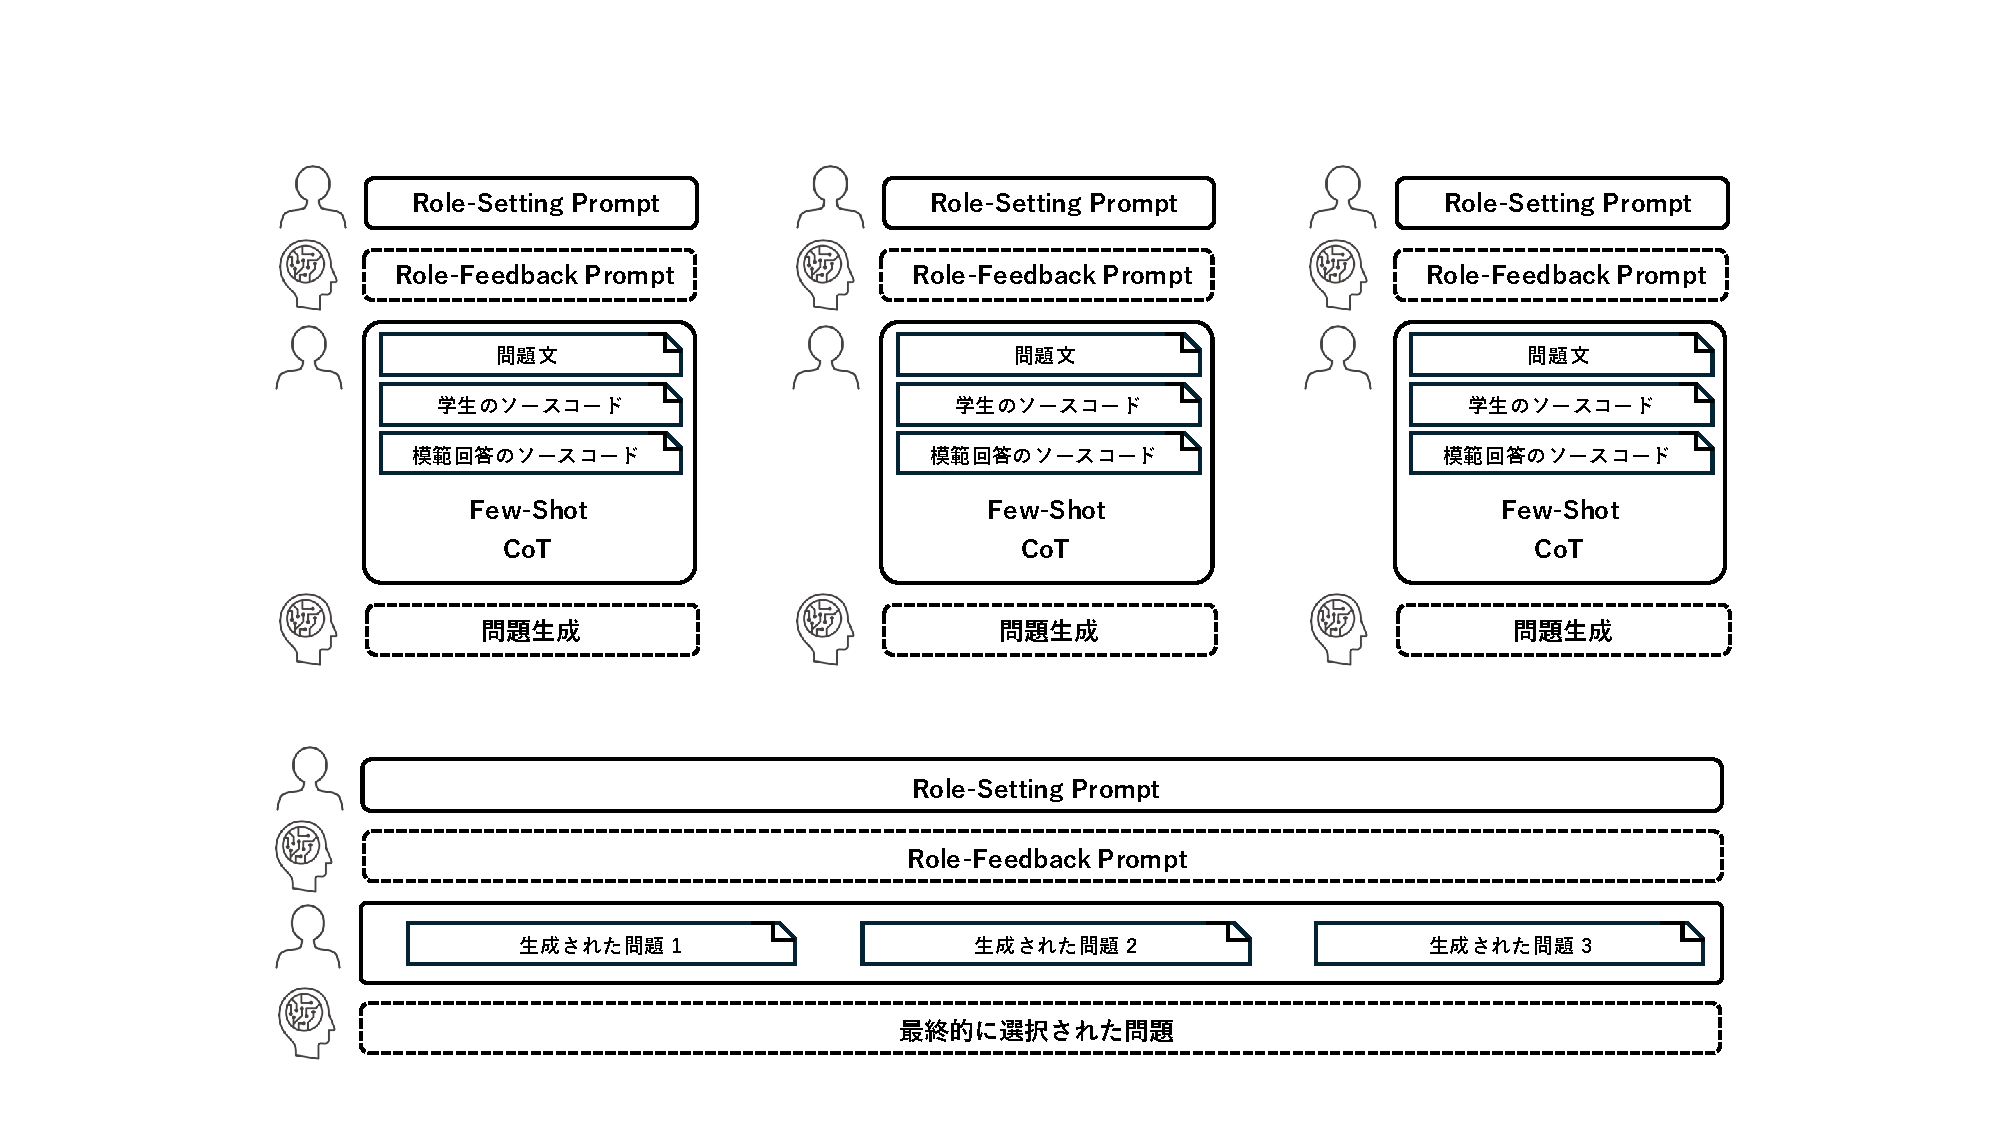
\includegraphics[width=1.0\linewidth]{figure/archtecture_figure_tlim.pdf}
    \caption{問題生成システムの概要図}
    \label{fig:system_overview}
\end{figure}

\subsection{役割付与とフィードバック指示}

まず,LLMに対してRole-Setting PromptとRole-Feedback Promptを付与し,プログラミング教師としての役割と,期待するフィードバックの種類を明確に伝える.これにより,LLMは以降の処理において教育的な観点からの分析と問題生成を行うように誘導される.

\subsection{Few-Shot Learning,CoTによる潜在スキル分析と問題生成}

問題生成の基盤として,Few-Shot Learningの手法を用いるとともに,学習者のソースコードから潜在的なスキルを分析するためにCoTを用いる.具体的には,プロンプト内に以下の情報を含める.

\begin{itemize}
    \item 学習者が過去に解答した問題文
    \item その問題に対する学習者のソースコード
    \item その問題に対する模範解答のソースコード
\end{itemize}

これらの情報とともに,LLMに対して,ソースコードのどの部分に着目し,どのような推論を経てスキルを判断したのかを段階的に出力するように指示する(CoT).これにより,LLMは学習者の解答傾向や誤りやすい箇所,模範的なコードの書き方などを学習し,個々の学習者に適した問題生成を行うための基礎情報を獲得するとともに,分析過程の透明性を高め,より質の高い問題生成に繋げる.また,Few-Shotの例には,学生のレベルやソースコードに対する評価値と評価内容などといった情報を含めることで,LLMはより適切な問題を選定・生成することが可能となる.例えば,「このコードではループ処理が適切に使用されていないため,ループの理解が不足している可能性がある」といった具体的な分析結果を出力させる.この分析結果に基づき,LLMは具体的な問題文を生成する.


\subsection{Self-Consistencyによる問題の選定と最終出力}

Few-Shot LearningとCoTによる分析結果に基づき生成された複数の問題から,Self-Consistencyの考え方に基づき,同一の入力(学習者の解答例など)に対して独立に3つの問題を生成する.生成された問題はファイルに保存し,後の選定段階で使用する.最後に,生成された3つの問題を比較検討し,教育的な観点から最も適切な問題を最終的な出力として選定する.この際,再度Role-Setting PromptとRole-Feedback Promptを付与することで,LLMに教師としての役割を再認識させ,客観的な評価を促す.問題の選定基準としては,問題の難易度が学習者のスキルレベルに合致しているか,問題文が明確で曖昧な点がないか,問題が独創的で学習意欲を刺激するか,などが挙げられる.選定された問題は学習者に提示される.


\section{本研究で使用したLLM}
本研究では,性能特性の異なる3種のLLMを比較評価する.図\ref{fig:system_overview}に示す共通のプロンプトを各LLMへの入力として用い,生成された問題を評価することで,各LLMの特性を分析する.以下では,各LLMの概要について述べる.
\begin{itemize}
\item \textbf{Gemini 1.5 Flash} (Google): 大規模なテキストおよびコードベースの文脈理解に優れている.
\item \textbf{GPT-4o mini} (OpenAI): 比較的軽量な構成ながら,高速な推論処理と多様なタスクへの適応性を特徴とする.
\item \textbf{GPT-4o} (OpenAI): 高度な推論能力とマルチモーダル処理機能を備え,4o-miniと比較してより精緻な自然言語処理が可能である.
\end{itemize}
各LLMの生成した問題の評価は,プログラミング学習者(以下,被験者とする)に実際に問題を解答させ,その解答コードとアンケート調査の結果に基づいて行う.本評価では,解答コードの正確性や効率性などを分析するとともに,アンケート調査を通じて被験者の主観的な評価を収集する.アンケート調査結果において使用した統計手法は第5章,ソースコードの分析やアンケートの分析など,実験の詳細な結果は第6章でそれぞれ詳述する.

\chapter{プロンプトエンジニアリング手法}
本章では,問題作問システムの構築に用いた4つのプロンプトエンジニアリング手法について詳述する.
\section{Role-Play Prompting}
2023年8月にKong et al.\cite{Role_play}によって提案されたRole-Play Promptingは,大規模言語モデル(LLM)のZero-Shot推論能力を効果的に向上させるためのプロンプトエンジニアリング手法である.この手法は,LLMに特定の役割を付与し,その役割に沿った応答を生成させることで,より高度な推論を引き出すことを目的としている.図\ref{fig:role-play-comparison}は,Role-Play PromptingとZero-Shotの手法を比較したものである.

Role-Play Promptingの中核となるのは,二段階のフレームワークである.第一段階では,タスクに特化した役割を定義するプロンプトであるRole-Setting Promptと,役割に対するフィードバックを行うプロンプトであるRole-Feedback Promptを構築する.Role-Setting Promptは,LLMに特定の役割を明示的に指示するものであり,例えば数学の問題を解く場合には,「あなたは優秀な数学教師です.」といったプロンプトを用いる.Role-Feedback Promptは,LLMの応答が役割に合致しない場合に,適切なフィードバックを与えるためのものである.第二段階では,第一段階で構築されたプロンプトを用いて,実際の質問に対する回答を生成する.この二段階のアプローチにより,LLMは与えられた役割の文脈に沿って推論を行うことが可能となる.

Kong et al.は,本手法の有効性を定量的に評価するため,12種類のベンチマークデータセットを用いた包括的な実験を実施した.これらのデータセットは,算術推論(例:AQuA),常識的推論(例:CommonsenseQA),記号推論(例:Symbolic Reasoning),およびその他の推論タスク(例:Last Letter)の4つのカテゴリーに分類される.実験では,OpenAIのChatGPTをベースモデルとして採用し,従来のZero-Shotプロンプティング手法およびZero-Shot Chain-of-Thought(CoT)プロンプティング手法との比較評価を行った.

実験結果は,Role-Play Promptingの有効性を明確に裏付けている.12のデータセットのうち10のデータセットにおいて,従来のZero-Shotプロンプティング手法を大幅に上回る性能を示した.特に,AQuAデータセットでは正解率が53.5\%から63.8\%へと10.3ポイント向上し,Last Letterデータセットでは23.8\%から84.2\%へと60.4ポイントという顕著な向上を記録した.さらに,Zero-Shot CoTプロンプティングと比較した場合でも,12のデータセット中9つのデータセットでRole-Play Promptingが優位性を示した.

注目すべき点として,Role-Play PromptingはLLMにおける暗黙的なChain-of-Thought(CoT)の生成を促進する効果があることが示唆された.特に,LLMが自発的にCoTを生成することが困難なタスクにおいて,役割の付与は思考の連鎖を誘導し,より論理的で詳細な推論プロセスを導くことが観察された.これは,役割がLLMに対して特定の思考様式を促し,問題解決のための段階的なアプローチを自然に生成させるためと考えられる.

手法の汎用性を検証するため,研究チームはLlama 2-Chat,Vicunaなど,異なるアーキテクチャとパラメータ数を持つ複数のオープンソース会話型LLMを用いた追加実験を実施した.その結果,モデルの規模(7Bから70Bパラメータまで)や種類に関わらず,Role-Play Promptingによる性能向上が一貫して確認された.この結果は,提案手法が特定のモデルアーキテクチャに依存しない,普遍的な有効性を持つ可能性を示唆している.

プロンプト設計の詳細な分析も行われ,役割の選択がモデルの性能に大きな影響を与えることが明らかになった.タスクの性質と合致する適切な役割(例えば,数学の問題に対して「優秀な数学教師」の役割)を選択することで,より高い性能が達成されることが示された.
\begin{figure}[tp]
    \centering
    \subfigure[Zero-Shot]{
        \fbox{%
            \begin{minipage}{0.95\textwidth}
                \textbf{入力} \\
                \textbf{ユーザー:} Xavierは4フィートの身長で3インチ成長しました.Coleは50インチの身長で夏の間に2インチ成長しました.ColeとXavierの身長差は今どれくらいですか?\\[2mm]
                \textbf{出力} \\
                \textbf{アシスタント:} Xavierの身長は4フィート + 3インチ = 7インチです.Coleの身長は50インチ + 2インチ = 52インチです.二人の身長差は52インチ - 7インチ = 45インチです.
            \end{minipage}%
        }
    }

    \vspace{5mm}

    \subfigure[Role-Play Prompting]{
        \fbox{%
            \begin{minipage}{0.95\textwidth}
                \textbf{入力} \\
                \textbf{ユーザー:} これからあなたは優秀な数学教師として,生徒に数学の問題を正確に教えていただきます.私はあなたの生徒の一人です.\\[2mm]
                \textbf{アシスタント:} はい,わかりました!数学の教師として,あなたが理解しやすいように数学の概念を正確に説明いたします.数学の問題や質問がありましたら,お気軽にどうぞ.一緒に数学の世界を探求していきましょう!\\[2mm]
                \textbf{ユーザー:} Xavierは4フィートの身長で3インチ成長しました.Coleは50インチの身長で夏の間に2インチ成長しました.ColeとXavierの身長差は今どれくらいですか?\\[2mm]
                \textbf{アシスタント:} ...1フィートは12インチなので,Xavierの初期身長は: 4フィート × 12インチ/フィート = 48インチです.3インチ成長したので,Xavierの新しい身長は: 48インチ + 3インチ = 51インチです....Coleの新しい身長は2インチ成長して: 50インチ + 2インチ = 52インチです....Xavierの身長をColeの身長から引くと: 52インチ - 51インチ = 1インチです.したがって,現在のColeとXavierの身長差は1インチです.
            \end{minipage}%
        }
    }

    \caption{Zero-ShotとRole-Play Promptingの比較例\\(Kong et al.~\cite{Role_play}のFigure 1を日本語に翻訳)}
    \label{fig:role-play-comparison}
\end{figure}
\section{Chain-of-Thought (CoT)}
Chain-of-Thought(CoT)Promptingは,大規模言語モデル(LLM)の推論能力,特に多段階の推論を必要とするタスクにおける性能を向上させるためのプロンプトエンジニアリング手法として,2022年にWei et al.\cite{CoT}が発表した.従来のプロンプティングでは,質問と回答のみを提示するのに対し,CoT Promptingでは,モデルに中間的な推論ステップを生成するように促すことで,より正確な結果を得ることを目的とする.

CoT Promptingでは,few-shot promptingと組み合わせて,回答に至るまでの思考過程の例をプロンプトに含めることで,LLMに段階的な思考過程を示すよう促す.プロンプトに「Let's think step by step」のようなフレーズを含めることは,CoT Promptingの一つの方法であるが,必須ではない.重要なのは,モデルに段階的な推論の例を示すことである.これにより,モデルは問題解決のプロセスを明示的に示しながら最終的な回答に至ることができる.特に,算術,常識的推論,記号操作,プログラム実行など,複数のステップを要する推論タスクにおいて,その効果が顕著に表れる.

本手法の有効性を検証するため,研究チームはBIG-Bench Hard(BBH)と呼ばれる,従来の評価において人間の平均的な性能を下回っていた,難易度の高い23のタスクセットを用いて実験を行った.これらのタスクは,LLMの推論能力を試すために特別に設計されたものである.実験では,GoogleのPaLMやOpenAIのCodexなどの大規模言語モデルをベースモデルとして使用し,標準的なZero-Shotプロンプティング手法と比較評価を実施した.

実験結果は,CoT Promptingの有効性を示している(表\ref{tab:cot-results}).特に,大規模な言語モデルにおいて,CoT Promptingは顕著な性能向上をもたらした.Wei et al.の研究では,PaLM 540Bモデルにおいて,BBHベンチマークの多くのタスクで大幅な性能向上が確認された.23のタスクのうち,17のタスクで人間の平均的な性能を上回る結果を達成したことは特筆に値する.

さらに,実験では,CoT Promptingの効果がモデルのサイズに大きく依存することも明らかになった.小規模なモデルでは,CoT Promptingは必ずしも性能を向上させず,場合によっては性能を低下させる可能性もある.しかし,モデルのパラメータ数が増加するにつれて,CoT Promptingの効果が顕著になり,大幅な性能向上が見られることが示された.Weiらの研究では,PaLMの8Bから540Bまでの異なるパラメータサイズのモデルで実験が行われ,モデルサイズと性能向上の間に明確な相関関係が示された.

CoT Promptingの汎用性を検証するため,他の研究ではLlama 2-ChatやVicunaなどのオープンソースの会話型LLMでも実験が行われている.これらの研究では,モデルの種類や規模,そしてタスクによって効果の程度は異なるものの,CoT Promptingが一定の性能向上をもたらす傾向が示されている.
\begin{table}[tp]
\centering
\small
\caption{大規模言語モデルのBIG-Bench Hard評価における手法別性能評価結果\\(Kong et al.~\cite{CoT}のTable 2を日本語に翻訳)}
\label{tab:cot-results}
\setlength{\tabcolsep}{4pt}
\begin{tabular}{@{}lcccl@{}}
\hline
& \begin{tabular}[c]{c}評価対象全体\\(23タスク)\end{tabular} 
& \begin{tabular}[c]{c}自然言語系\\(12タスク)\end{tabular} 
& \begin{tabular}[c]{c}アルゴリズム系\\(11タスク)\end{tabular} 
& \begin{tabular}[c]{c}平均人間性能\\超過タスク数\end{tabular} \\
\hline
人間性能(平均) & 67.7 & 71.2 & 63.5 & N/A \\
人間性能(最高) & 94.4 & 92.2 & 96.9 & 23 / 23 \\
既存手法による最高性能 & 50.9 & 60.5 & 40.3 & 0 / 23 \\
\hline
\multicolumn{5}{@{}l}{\bf PaLM 540B} \\
従来型プロンプティング & 52.3 & 62.7 & 40.9 & 6 / 23 \\
Chain-of-Thought & 65.2 (+12.9) & 71.2 (+8.5) & 58.6 (+17.7) & 10 / 23 \\
\hline
\multicolumn{5}{@{}l}{\bf InstructGPT} \\
従来型プロンプティング & 51.8 & 60.9 & 42.0 & 4 / 23 \\
Chain-of-Thought & 68.4 (+16.6) & 71.3 (+10.4) & 65.3 (+23.3) & 15 / 23 \\
\hline
\multicolumn{5}{@{}l}{\bf Codex} \\
従来型プロンプティング & 56.6 & 66.4 & 45.9 & 5 / 23 \\
Chain-of-Thought & 73.9 (+16.7) & 73.5 (+7.1) & 74.4 (+28.5) & 17 / 23 \\
\hline
\end{tabular}
\end{table}

\section{Few-Shot Learning}
2020年に発表されたGPT-3の論文\cite{Few-shot}において示されたFew-Shot Learningは,大規模言語モデルにおける重要な学習パラダイムの一つである.従来の機械学習手法では,特定のタスクに対して数千から数十万規模の学習データを用いたファインチューニングが不可欠であった.対照的に,Few-Shot Learningでは,数例から数十例程度のデモンストレーションをコンテキストとして与えるのみで,モデルが新たなタスクに迅速に適応することが可能となる(図\ref{fig:learning-strategies}).

具体的なメカニズムとしては,モデルのコンテキストウィンドウ内に,タスクの説明文と少数の例示を包含する.その後,新たな入力に対する予測を行う際,モデルはこれらの例示を参照することで,タスクの本質を把握し,適切な出力を生成する.GPT-3の実験では,通常10から100例程度の例示が用いられ,これはモデルのコンテキストウィンドウサイズ(2048トークン)によって制約を受ける.

GPT-3を用いた実験を通じて,Few-Shot Learningの有効性は複数のタスクにおいて実証されている.特筆すべき成果として,TriviaQAタスクにおいては,Few-Shot設定で71.2\%の精度を達成し,同一のクローズドブック設定における事前学習済みモデルの最高性能を凌駕した.また,LAMBADAデータセットにおいては,Few-Shot設定で86.4\%の精度を記録し,従来の最高性能を18\%上回る顕著な結果を示した.

さらに,算術演算や単語アナグラムといった基本的な推論タスクにおいても,Few-Shot Learningは有効に機能することが示された.例えば,2桁の加算タスクでは100\%の正確性を達成し,3桁の加算においても80.2\%の正確性を示した.これらの結果は,モデルが単なる記憶に留まらず,実際の計算能力を獲得している可能性を示唆している.

興味深いことに,モデルの規模拡大に伴い,Few-Shot Learningの性能が向上する傾向が観察された.これは,モデルの規模拡張によって,より高度な文脈適応能力が獲得されることを示唆している.特に,GPT-3の175Bパラメータモデルは,より小規模なモデルと比較して,際立って優れたFew-Shot Learning能力を示した.

\begin{figure}[tp]
\centering
\begin{tikzpicture}[
    box/.style={draw, rectangle, minimum width=7cm, minimum height=2cm, align=left},
    arrow/.style={->, thick},
    note/.style={font=\small\itshape, align=center}
]
    % 各ボックスの間隔設定
    \def\boxsep{3.5cm}

    % ゼロショット学習
    \node[box] (zero) at (0, \boxsep*2) {
        \textbf{Zero-Shot Learning}\\
        入力: 「サービスは素晴らしかった!」\\
        \textcolor{gray}{$\rightarrow$ 事前例なしで予測}
    };

    % ワンショット学習
    \node[box] (one) at (0, \boxsep*1) {
        \textbf{One-Shot Learning}\\
        例: 「最悪の体験」 $\rightarrow$ ネガティブ\\
        入力: 「サービスは素晴らしかった!」\\
        \textcolor{gray}{$\rightarrow$ 単一例から学習}
    };

    % フューショット学習
    \node[box] (few) at (0, 0) {
        \textbf{Few-Shot Learning}\\
        例1: 「最悪の体験」 $\rightarrow$ ネガティブ\\
        例2: 「素晴らしい!」 $\rightarrow$ ポジティブ\\
        例3: 「がっかりする」 $\rightarrow$ ネガティブ\\
        入力: 「サービスは素晴らしかった!」\\
        \textcolor{gray}{$\rightarrow$ 複数例から学習}
    };

    % 左側のラベル
    \node[note] at (-5.5, \boxsep*2) {例なし};
    \node[note] at (-5.5, \boxsep*1) {1つの例};
    \node[note] at (-5.5, 0) {複数の例};

    % ボックスを接続する矢印
    \draw[arrow] (zero.south) -- (one.north);
    \draw[arrow] (one.south) -- (few.north);

\end{tikzpicture}
\vspace{0.5cm} % タイトルを下げる
\caption{言語モデルにおける学習アプローチの進化}
\label{fig:learning-strategies}
\end{figure}


\section{Self-Consistency}
2022年にWang et al.\cite{Self-consitency}によって提案されたSelf-Consistencyは,Chain-of-Thought (CoT) プロンプティングと組み合わせることで,大規模言語モデル(LLM)の推論能力を向上させる手法である.

Self-Consistencyの基本的な着想は,複雑な推論問題に対して,通常,正解に至る複数の異なる思考経路が存在するという洞察に基づいている.本手法では,言語モデルのデコーダーから複数の推論経路をサンプリングし,それらの中で最も一貫性のある答えを選択する.具体的には,まずCoTプロンプティングを用いて言語モデルに推論過程を生成させる.次に,単一の貪欲なデコーディングではなく,複数の異なる推論経路をサンプリングする.各推論経路は異なる最終的な答えに帰着する可能性があるが,正当な推論プロセスは,多様な経路を経由したとしても,同一の正解に収束する傾向がある.

実験結果は,Self-Consistencyの有効性を明確に示している.UL2-20B,GPT-3-175B,LaMDA-137B,PaLM-540Bという4つの異なる言語モデルを用いた評価では,算術推論や常識推論を含む広範なタスクにおいて,CoTプロンプティングと比較して大幅な性能向上が確認された.特に,GSM8K(+17.9\%),SVAMP(+11.0\%),AQuA(+12.2\%),StrategyQA(+6.4\%),ARC-challenge(+3.9\%)における精度向上が顕著である.

本手法の重要な特徴は,追加の学習や人手によるアノテーションを必要としない点である.既存の事前学習済み言語モデルに対してそのまま適用可能であり,補助モデルやファインチューニングも不要である.また,モデルアンサンブルとは異なり,単一のモデルで「自己アンサンブル」として機能する.

実験では,サンプリング戦略やパラメータに対する堅牢性も検証された.温度サンプリング,top-kサンプリング,核サンプリングなど,多様なデコーディング手法において一貫した改善が見られた.さらに,サンプリングする推論経路の数を増加させることで,性能が安定的に向上することも示されている.

Self-Consistencyは,不完全なプロンプトや自然言語以外の推論経路(例えば,数式など)に対しても有効であり,ゼロショットCoTと組み合わせた場合でも顕著な改善(+26.2\%)を示した.本手法の制約は計算コストの増加のみであるが,少数のパス(5-10程度)でも大部分の改善を実現できることが確認されている.

\begin{figure}[t]
\centering
\begin{tikzpicture}[
 box/.style={draw, rectangle, minimum width=4cm, minimum height=1.2cm, align=center},
 arrow/.style={->, >=latex}, 
 node distance=2cm
]

% 入力問題
\node[box] (input) at (0,6) {
問題:駐車場に3台の車があり,\\
新たに2台が到着した場合,\\
合計何台になりますか?
};

% 言語モデル
\node[box] (lm) at (0,4) {言語モデル};

% 複数の推論経路(左右に分散配置)
\node[box] (path1) at (-5,2) {
経路1: 駐車場には3台あり\\
2台追加で合計3 + 2 = 5台\\
答え: 5
};

\node[box] (path2) at (0,2) {
経路2: 最初の3台に\\
2台を加えると5台\\
答え: 5
};

\node[box] (path3) at (5,2) {
経路3: 現在の3台から\\
さらに2台で計5台\\
答え: 5
};

% 最終結果
\node[box] (result) at (0,0) {最も一貫性のある回答: 5台};

% 矢印
\draw[arrow] (input) -- (lm);
\draw[arrow] (lm) -- (path1);
\draw[arrow] (lm) -- (path2);
\draw[arrow] (lm) -- (path3);
\draw[arrow] (path1) -- (result);
\draw[arrow] (path2) -- (result);
\draw[arrow] (path3) -- (result);

\end{tikzpicture}
\vspace{0.5cm} % タイトルを下げる
\caption{Self-Consistencyによる推論過程\\(Wang et al.~\cite{Self-consitency} の Figure 1 を参考)}
\label{fig:self-consistency}
\end{figure}
\chapter{評価時における分析手法}
\section{一元配置分散分析}
一元配置分散分析は,3つ以上の群の平均値を比較するための統計手法である.ある要因(因子)が量的変数に与える影響を評価する際に用いられる.例えば,異なる肥料が作物の収穫量に与える影響を検証する場合などが該当する.

分散分析の基本的な考え方は,「群間の変動」と「群内の変動」を比較することにある.群間の変動が群内の変動に比べて十分に大きければ,要因が変数に有意な影響を与えていると判断する.

具体的には,以下の手順で分析を行う.

\begin{enumerate}
    \item \textbf{平方和の計算:}
    \begin{itemize}
        \item \textbf{全平方和 (SST):} 全てのデータと全体の平均値の差の二乗和.
        \begin{equation}
        SST = \sum_{i=1}^{k} \sum_{j=1}^{n_i} (x_{ij} - \bar{x})^2
        \end{equation}
        ここで,$x_{ij}$ は $i$ 群の $j$ 番目のデータ,$n_i$ は $i$ 群のサンプルサイズ,$\bar{x}$ は全体の平均値,$k$ は群の数である.
        \item \textbf{群間平方和 (SSB):} 各群の平均値と全体の平均値の差の二乗和.
        \begin{equation}
        SSB = \sum_{i=1}^{k} n_i (\bar{x}_i - \bar{x})^2
        \end{equation}
        ここで,$\bar{x}_i$ は $i$ 群の平均値である.
        \item \textbf{群内平方和 (SSW):} 各群のデータとそれぞれの群の平均値の差の二乗和.
        \begin{equation}
        SSW = \sum_{i=1}^{k} \sum_{j=1}^{n_i} (x_{ij} - \bar{x}_i)^2
        \end{equation}
        SST = SSB + SSW の関係が成り立つ.
    \end{itemize}
    \item \textbf{自由度の計算:}
    \begin{itemize}
        \item 群間自由度 (dfB): $df_B = k - 1$
        \item 群内自由度 (dfW): $df_W = N - k$ (ここで $N$ は全体のサンプルサイズ)
    \end{itemize}
    \item \textbf{平均平方の計算:}
    \begin{itemize}
        \item 群間平均平方 (MSB): $MSB = \frac{SSB}{df_B}$
        \item 群内平均平方 (MSW): $MSW = \frac{SSW}{df_W}$
    \end{itemize}
    \item \textbf{$F$値の計算:}
    \begin{equation}
    F = \frac{MSB}{MSW}
    \end{equation}
\end{enumerate}

この$F$値と事前に設定した有意水準 ($\alpha$) に基づいて,F分布表を参照し,帰無仮説(全ての群の母平均は等しい)を棄却するかどうかを判断する.$F$値が大きければ大きいほど,群間に差がある可能性が高くなる.具体的には,$F$値に対応する$p$値を求め,$p$値が$\alpha$以下であれば帰無仮説を棄却する.

ただし,一元配置分散分析は各群のデータが正規分布に従うこと,および各群の分散が等しいこと(等分散性)を前提としている.等分散性の検定には,例えばLevene検定などが用いられる.これらの前提が満たされない場合は,ノンパラメトリック検定(例えばKruskal-Wallis検定)を検討する必要がある.有意な差が認められた場合は,どの群間に差があるのかを特定するために,事後検定(例えばTukeyのHSD検定(5.2
節),Bonferroni補正など)が必要となる.

本研究では,各モデルが生成した問題に対する評価を比較するため,アンケート調査の各指標に対して一元配置分散分析を用いた.

\section{TukeyのHSD検定}
TukeyのHSD検定は,分散分析において群間に有意な差が認められた後に,どの群間に具体的な差があるのかを特定するための事後検定(多重比較検定)の一つである.特に,全ての群のペアについて比較を行う場合に適している.HSDは "Honestly Significant Difference" の略であり,全ての対比較において第一種の過誤(実際には差がないのに差があると判断してしまう過ち)を一定の水準(通常は$\alpha = 0.05$)に制御することを目的としている.

TukeyのHSD検定は,以下の手順で行われる.

\begin{enumerate}
    \item \textbf{スチューデント化された範囲 ($q$) の計算:}

    各群の平均値の差を,群内変動の標準誤差で割ることで,スチューデント化された範囲 $q$ を計算する.

    \begin{equation}
    q = \frac{|\bar{x}_i - \bar{x}_j|}{SE}
    \end{equation}

    ここで,$\bar{x}_i$ と $\bar{x}_j$ は比較する2つの群の平均値,$SE$ は群内変動の標準誤差であり,以下のように計算される.

    \begin{equation}
    SE = \sqrt{\frac{MSW}{n}}
    \end{equation}

    ここで,$MSW$ は分散分析で計算された群内平均平方,$n$ は各群のサンプルサイズ(群のサンプルサイズが異なる場合は,調和平均を用いる).

    \item \textbf{有意差の判定:}

    計算された $q$ 値を,スチューデント化された範囲の分布表と比較する.この分布表は,群の数と群内自由度 ($df_W$) によって値が異なる.比較の結果,計算された $q$ 値が分布表の値よりも大きければ,その2つの群間には有意な差があると判断する.あるいは,$p$値を計算し,事前に設定した有意水準 ($\alpha$) と比較する方法もある.$p$値が$\alpha$以下であれば,その2つの群間には有意な差があると判断する.
    
\end{enumerate}

TukeyのHSD検定は,全ての対比較を行うため,他の多重比較検定(例えばBonferroni補正)に比べて検出力が高い反面,第一種の過誤を犯す可能性が若干高くなる.しかし,全てのペアを比較する必要がある場合には,適切な方法である.

例えば,ある研究で4つの異なる教授法(A, B, C, D)の効果を比較するために実験を行い,分散分析の結果,教授法間に有意な差が認められたとする.この場合,TukeyのHSD検定を用いることで,AとB,AとC,AとD,BとC,BとD,CとDという全ての教授法のペアについて,どのペア間に有意な差があるのかを具体的に明らかにすることができる.

本研究では,一元配置分散分析によってモデル間に有意な差が認められた評価指標について,TukeyのHSD検定を用いてどのモデル間に差があるのかを特定した.


\chapter{計算機実験}
\section{概要}
本研究では,提案するLLMを用いた問題生成手法の有効性を検証するため,比較実験を実施した.具体的には,提案手法を3種類の異なるLLMに入力として与え,プログラミング問題を生成させた.生成された問題の質および教育的効果を評価するため,実際にプログラミングを学習中の学生である被験者に問題への解答を依頼し,その結果を分析した.さらに,被験者に対してアンケートを実施し,生成された問題に対する主観的な評価を収集した.これらの客観的な解答結果と主観的なアンケート結果を統合的に分析することで,各LLMが生成する問題の特性を比較評価し,提案手法の有効性を多角的に検証することを目的とした.実験に用いたアンケートの詳細については6.2節に,被験者が作成したソースコードに対する分析の詳細については6.3節に,実験で使用したデータセットの詳細については6.4節に,そして実験結果の詳細については6.5節にそれぞれ記述する.この実験構成により,生成された問題の妥当性,被験者の解答状況,および被験者による評価を総合的に分析し,提案手法の有効性を実証的に評価することを意図している.
\section{アンケートの詳細}
本研究では,LLMが生成した問題に対する学生の評価を多角的に収集するため,問題解答後にアンケートを実施した.被験者である学生には,以下の6つの質問項目に対して10段階評価(星1:最低評価,星10:最高評価)で回答を求めた.これらの質問項目は,生成された問題の様々な側面,すなわち明確性,学習効果,難易度,興味深さ,質,および解答時間に関する評価を捉えることを目的としている.なお,各問題の解答時間として15分を設定しているが,これは分析に用いたデータの一つひとつが約15分の解答を想定して作成されていることに基づいている.データの詳細については6.4節を参照されたい.

\subsection{アンケート項目}

\begin{itemize}
    \item \textbf{問題の文章は理解しやすかったですか?} (星1:わかりにくい,星10:わかりやすい)
    \item \textbf{新しいことを学ぶ機会になりましたか?} (星1:ならない,星10:なった)
    \item \textbf{難易度はどうでしたか?} (星1:簡単すぎる,星10:難しすぎる)
    \item \textbf{この問題を解いて,楽しかったですか?} (星1:つまらなかった,星10:楽しかった)
    \item \textbf{「いい問題だな」と思いましたか?} (星1:あてはまらない,星10:あてはまる)
    \item \textbf{この問題の解答時間である15分は適切でしたか?} (星1:短かった,星10:長かった)
\end{itemize}

\subsection{設問意図}

上記の各設問には,以下のような意図がある.

\begin{itemize}
    \item \textbf{理解しやすさ}(問題の文章は理解しやすかったですか?) \\この質問は,問題文の明確性を評価することを目的としている.問題文が曖昧であったり,専門用語が多用されていたりする場合,学生は問題を正しく理解することができず,解答に支障をきたす可能性がある.この質問を通して,LLMが生成する問題文が学生にとって理解しやすいか,つまり,問題の意図が適切に伝わるかを検証する.
    \item \textbf{新しい学び}(新しいことを学ぶ機会になりましたか?) \\この質問は,問題が学生の学習に貢献したかどうかを評価することを目的としている.良質な問題は,学生に新しい知識や考え方を習得する機会を提供する.この質問を通して,LLMが生成する問題が学生にとって新たな学びの機会となっているかを検証する.
    \item \textbf{難易度}(難易度はどうでしたか?) \\この質問は,問題の難易度が適切かどうかを評価することを目的としている.難易度が高すぎると学生は挫折しやすく,低すぎると学習効果が得られない.この質問を通して,LLMが生成する問題の難易度が学生のレベルに合致しているかを検証する.
    \item \textbf{楽しさ}(この問題を解いて,楽しかったですか?) \\この質問は,問題が学生の学習意欲を高めるかどうかを評価することを目的としている.楽しく取り組める問題は,学習効果を高めることが期待される.この質問を通して,LLMが生成する問題が学生にとって興味深く,学習意欲を刺激するものであるかを検証する.
    \item \textbf{良問評価}(「いい問題だな」と思いましたか?)\\この質問は,問題の総合的な質を評価することを目的としている.この質問は,問題の明確性,適切性,難易度,興味深さなど,様々な要素を包括的に評価する役割を果たすと考えられる.学生が「いい問題だな」と感じるかどうかは,問題の総合的な魅力や教育的価値を反映していると考えられるため,重要な評価指標となる.
    \item \textbf{時間の適切さ}(この問題の解答時間である15分は適切でしたか?)\\この質問は,問題の解答に要する時間が適切かどうかを評価することを目的としている.解答時間が短すぎると十分に問題を考えることができず,長すぎると集中力が途切れる可能性がある.この質問を通して,LLMが生成する問題に対して設定された解答時間が適切であったかを検証する.15分という問題設定は分析で使用したデータの一つひとつが約15分想定であることを加味している.データの詳細ついては6.4節を参照のこと.
\end{itemize}

これらの質問を通して得られた回答は,第5章で提示した分析手法を用いて分析を行い,LLMが生成する問題の質を多角的に評価するための重要なデータとなる.具体的には,各質問項目に対する平均点や標準偏差を算出し,LLM間の比較や,理想的な問題とのギャップなどを分析することが考えられる.また,質問項目間の相関分析を行うことで,問題の明確性や難易度などが学習効果や興味深さにどのように影響するかを考察することも可能である.

\section{ソースコード解析}
本研究では,LLMが生成した問題に対する学生の解答コードを客観的に評価するため,GPT-4oを用いたコード評価を実施した.GPT-4oを採用した主な意図は,LLMが持つ高度なコード理解能力を活用することで,人間による評価と同等またはそれ以上の精度で,かつ効率的にコードの品質を評価することにある.特に,コードの正確性,効率性,可読性,およびプログラミング概念の理解といった多角的な視点からの評価を,一貫性を持って行うことを目的としている.

評価は以下の4項目について,5段階評価で行った.

\subsection{評価項目}

\begin{enumerate}
    \item \textbf{正確性:コードの正確性と問題解決力} \\
    この項目は,コードが問題の要件をどれだけ正確に満たし,問題を解決できているかを評価する.
    \begin{itemize}
        \item 5点: 完全に正確で,すべての要件を満たし,エッジケースも考慮されている.
        \item 4点: ほぼ正確で,主要な要件を満たしている.
        \item 3点: 基本的な機能は動作するが,一部に問題がある.
        \item 2点: 大きな問題があり,要件を十分に満たさない.
        \item 1点: ほとんど機能しない.
    \end{itemize}
    \item \textbf{効率性:コードの効率性} \\
    この項目は,コードの実行効率,すなわちアルゴリズムの選択や実装の最適性を評価する.
    \begin{itemize}
        \item 5点: 最適なアルゴリズムと実装が用いられている.
        \item 4点: 効率的な実装だが,改善の余地がある.
        \item 3点: 標準的な効率性である.
        \item 2点: 非効率な実装が目立つ.
        \item 1点: 著しく非効率である.
    \end{itemize}
    \item \textbf{可読性:コードの可読性とスタイル} \\
    この項目は,コードの読みやすさ,命名規則の適切さ,構造の整理などを評価する.
    \begin{itemize}
        \item 5点: 極めて読みやすく,整理された構造を持っている.適切なコメントやドキュメンテーションも含まれている.
        \item 4点: 読みやすく,適切な命名と構造化がなされている.
        \item 3点: 基本的な可読性は確保されている.
        \item 2点: 読みにくい部分が多い.コメントやドキュメンテーションが不足している.
        \item 1点: ほとんど読めない.命名規則が不適切で,構造も整理されていない.
    \end{itemize}
    \item \textbf{基本概念:プログラミングの基本概念の理解} \\
    この項目は,コードがプログラミングの基本的な概念(変数,データ型,制御構造,関数など)を正しく理解し,適切に適用できているかを評価する.この項目を設けた意図は,単にコードが動作するかどうかだけでなく,学生がプログラミングの基礎をしっかりと理解しているかを評価することにある.表面的なコーディングだけでなく,根本的な理解度を測ることで,教育的な観点からの分析を深めることを目的としている.
    \begin{itemize}
        \item 5点: 言語機能を適切に使いこなせている.高度な概念も正しく理解し,応用できている.
        \item 4点: 基本概念を正しく理解し,適用できている.
        \item 3点: 基本的な理解は示しているが,一部不十分な点が見られる.
        \item 2点: 概念の理解が不十分で,誤用が見られる.
        \item 1点: 基本的な概念の誤用が目立つ.
    \end{itemize}
\end{enumerate}
図\ref{fig:base-prompt}は,本分析で使用するLLMへの入力プロンプトの設計概要を示している.分析に際しては,Role-Play Prompting(Role-Setting PromptとRole-feedback Promptで構成)を再定義し,プロンプトの冒頭に付与した.具体的なプロンプトの内容は,付録図\ref{fig:few-shot-examples}に示す.

これらの分析結果は,6.2節で紹介したアンケート結果と複合的に分析することで,多角的な評価を行う.アンケート結果から得られる主観的な評価と,ソースコード分析から得られる客観的な評価を組み合わせることで,LLMが生成する問題の教育的効果について,より深い洞察を得ることを目指す.
\section{実験データ}

本研究では,2024年度木更津工業高等専門学校情報工学科2年の「プログラミング基礎II」後期中間試験の問題と,試験に出席した学生41名が提出したソースコードをデータとして用いた.この試験は筆記試験を含む計7問で構成されており,本研究ではそのうち学生に実際にプログラミングをさせる3問を対象とした.各問題の問題文と問題を解くにあたって必要となるスキルを表\ref{tab:problems}に示す.

\begin{table}[h]
    \centering
    \caption{実験に用いたプログラミング問題}
    \label{tab:problems}
    \begin{tabular}{p{0.1\textwidth}p{0.7\textwidth}p{0.15\textwidth}}
        \toprule
        \textbf{問題ID} & \textbf{問題文} & \textbf{必要スキル} \\
        \midrule
        No.4.c & \begin{minipage}[t]{0.7\textwidth}
        以下の内容をすべて含むプログラムを作成しなさい.\\
        (1)キーボードから入力した数の分だけ,配列を動的に確保しなさい.その配列の要素として,0から99の値をランダムに入力しなさい.配列の要素をすべて出力しなさい.\\
        (2)その配列の要素を逆順に出力しなさい\\
        (3)その配列の要素の内,偶数だけ出力しなさい.
        \end{minipage} & 動的メモリ確保,配列操作,乱数生成,条件分岐 \\
        \midrule
        No.5.c & \begin{minipage}[t]{0.7\textwidth}
        以下の線形代数の行列に関するプログラムを作成せよ.\\
        (1)n行n列の正方行列Aを2次元配列として動的に確保しなさい.その要素として,0から9の値をランダムに入力して表示しなさい.動的に確保する2次元配列は,main関数内で行って構わない.\\
        (2)作成した行列Aの対角成分の和を求めなさい.\\
        (3)作成した行列Aの転置行列を求めなさい.ただし,転置行列は,(1)で作成した2次元配列に上書きしてから表示すること.
        \end{minipage} & 2次元配列の動的メモリ確保,行列演算 \\
        \midrule
        No.6.c & \begin{minipage}[t]{0.7\textwidth}
        2つの文字列を結合するプログラムを作成せよ.\\
        例えば char str1[] = "Kisarazu"; char str1[] = "City";の場合,結合するとKisarazuCityとなる.結合するために必要な配列は動的に確保すること.str1とstr2とは任意の文字列に対応すること.
        \end{minipage} & 文字列操作,動的メモリ確保 \\
        \bottomrule
    \end{tabular}
\end{table}

これらの問題文,学生が実際に解いたソースコード,および各問題に対して定義された模範解答のソースコードを用意し,実際の問題生成用プロンプトに組み込んだ.

なお,対象の学生の中には,これらの問題を全て解いていない者もいた.そこで,未解答の問題に対しては「未解答」のラベルを付与した.これにより,LLMが問題作成時に問題が解けないという事実からも学生のスキルを推定する材料としている.

\section{実験方法}
本研究では,6.4節で収集したデータを用いて,3.2節で紹介した3種類のLLMそれぞれにプログラミング問題の生成を依頼した.各LLMから学生一人ひとりに対応した問題が生成され,各学生に対して3種類の問題(各LLMから1問ずつ)が用意されることとなった.

生成された問題を用いた小テストは,情報工学科2年生を対象とした3回の授業の冒頭に実施した.各学生には事前に一意の匿名IDを付与しており,テストの配布時およびアンケートの収集時にはこのIDを使用した.これにより,回答の匿名性を確保することが可能となった.各テストの制限時間は15分とし,テスト終了後,各問題に対するアンケート調査を実施した.アンケートはGoogleフォームを用いて作成し,回答の際には配布されたIDを使用するよう指示した.

これらの実験を踏まえて,アンケートの結果と,実験の際に書いた学生のソースコードをGPT-4oで分析した結果を集約して,分析を行った.
\section{実験結果}

\subsection{各モデルのアンケート回答傾向}
各モデルのアンケート回答の平均値をMean(以下,$M$と表記する)として分析を行った.各モデルの特徴的な傾向として,Gemini 1.5 Flashは理解しやすさの平均値が最も高く $(M=7.40)$,評価指標間の相関も最も強く,問題の一貫性が高いことが示された.GPT-4o miniは,楽しさ $(M=6.55)$ と良問評価 $(M=6.63)$ において若干高い評価を得ており,学習者のモチベーションを高める問題生成に強みを持つ可能性がある.GPT-4oは全体的に中間的な評価を示し,バランスの取れた問題生成を行うと言える.

全モデルに共通する傾向として,「時間の適切さ」の評価が比較的低い値 $(M=4.34\sim4.56)$ を示した.これは,1に近いほど「問題を解く時間が短いと感じた」ことを意味するため,実験で設定した時間(15分)は,多くの被験者にとって短すぎたと解釈できる.また,ソースコード評価は全モデルで比較的低い値(2-3点台)を示しており,生成されたコードの品質には改善の余地があることが示された.

\begin{table}[htbp]
  \centering
  \caption{各モデルにおけるアンケート項目の平均値}
  \label{tab:mean_values}
  \begin{tabular}{lccc}
    \toprule
    アンケート項目 & Gemini 1.5 Flash & GPT-4o mini & GPT-4o \\
    \midrule
    理解しやすさ & 7.40 & 6.00 & 6.97 \\
    新しい学び & 5.69 & 5.37 & 5.89 \\
    難易度 & 5.51 & 4.92 & 5.75 \\
    楽しさ & 6.51 & 6.55 & 6.03 \\
    良問評価 & 6.43 & 6.63 & 6.22 \\
    時間の適切さ & 4.49 & 4.34 & 4.56 \\
    \bottomrule
  \end{tabular}
\end{table}

\newpage
\subsection{モデル比較(一元配置分散分析とTukeyのHSD検定)}

各モデルが生成した問題に対する評価を比較するため,アンケート調査の各指標に対して一元配置分散分析と TukeyのHSD 検定を実施した.アンケート調査における一元配置分散分析の結果を表\ref{tab:anova_results}に示す.


「理解しやすさ」において統計的に有意な差が確認された $(F=3.0928, p=0.0495)$.TukeyのHSD検定の結果,特にGemini 1.5 Flash とGPT-4o miniの間には有意差 $(p=0.0456)$ が認められ,Gemini 1.5 Flashが生成する問題は他のモデルと比較して最も理解しやすいという結果となった.この結果の詳細は表 \ref{tab:tukey_hsd_understanding} に示す.GPT-4oは両者の中間的な値を示したものの,有意な差は見られなかった.

他のアンケート指標(新しい学び,難易度,楽しさ,良問評価,時間の適切さ)においては,モデル間に統計的に有意な差は見られなかった.表\ref{tab:anova_results}は,アンケート調査における一元配置分散分析の結果を示す.

\begin{table}[h]
  \centering
  \caption{アンケート調査における一元配置分散分析の結果}
  \label{tab:anova_results}
  \begin{tabular}{lccc}
    \hline
    評価項目 & $F$値 & $p$値 & 有意性(5\%水準) \\
    \hline
    理解しやすさ & 3.0928 & 0.0495 & 有意差あり \\
    新しい学び & 0.3899 & 0.6781 & 有意差なし \\
    難易度 & 1.5028 & 0.2272 & 有意差なし \\
    楽しさ & 0.5317 & 0.5891 & 有意差なし \\
    良問評価 & 0.2966 & 0.7440 & 有意差なし \\
    時間の適切さ & 0.1000 & 0.9049 & 有意差なし \\
    \hline
  \end{tabular}
\end{table}

\begin{table}[h]
  \centering
  \caption{「理解しやすさ」におけるTukeyのHSD検定の結果}
  \label{tab:tukey_hsd_understanding}
  \begin{tabular}{lccccc}
    \hline
    比較 & 平均差 & $p$値 & 下限 & 上限 & 有意性(5\%水準) \\
    \hline
    GPT-4o vs. GPT-4o mini & -0.9722 & 0.2142 & -2.3406 & 0.3962 & 有意差なし \\
    GPT-4o vs. Gemini 1.5 Flash & 0.4278 & 0.7474 & -0.9689 & 1.8244 & 有意差なし \\
    GPT-4o mini vs. Gemini 1.5 Flash & 1.4000 & 0.0456 & 0.0216 & 2.7784 & 有意差あり \\
    \hline
  \end{tabular}
\end{table}

\subsection{各指標との相関分析}
表\ref{tab:correlation_results_all_detailed}は,各モデルにおけるアンケート調査指標とソースコード評価指標間の相関係数を示す.各モデルにおける評価指標間の相関分析を行った結果,特にGemini 1.5 Flashにおいて顕著な傾向が認められた.「難易度」(アンケート調査)と各ソースコード評価指標(正確性,効率性,可読性,基本概念)の間には強い負の相関 $(r=−0.657\sim−0.759)$ が観察された.これは,Gemini 1.5 Flashが生成する問題において,学生が難易度が高いと判断した問題ほど,コードの品質が低下する傾向を示している.また,「時間の適切さ」(アンケート調査)と各ソースコード評価指標の間には中程度の正の相関 $ (r=0.444\sim0.614) $ が見られ,問題に取り組む時間が適切であると感じるほど,コードの品質も向上する傾向が示唆された.さらに,「新しい学び」(アンケート調査)と各ソースコード評価指標の間には中程度の負の相関 $(r=−0.417\sim−0.566)$ が見られ,新しい学びが多いと感じるほど,コードの品質が低下する傾向が示された.これは,新しい概念を学習する際に,コードの完成度よりも学習に重点が置かれるためと考えられる.

一方,他のモデル(GPT-4oおよびGPT-4o mini)においては,上記のような顕著な相関関係は見られなかった.いくつかの指標間には弱い相関が見られたものの,Gemini 1.5 Flashで見られたような強い負の相関や中程度の正の相関は確認されなかった.このことから,上記の傾向は特にGemini 1.5 Flashに特有の傾向であると考えられる.

\begin{table}[t]
  \centering
  \caption{各モデルにおけるアンケート調査指標とソースコード評価指標間の相関係数}
  \label{tab:correlation_results_all_detailed}
  \begin{threeparttable}
    \begin{tabular}{lcccc}
      \hline
      評価指標の比較\\(アンケートvs.ソースコード) & Gemini 1.5 Flash & GPT-4o mini & GPT-4o\\
      \hline
    理解しやすさ vs. 正確性 & 0.328 & -0.059 & 0.064 \\
    理解しやすさ vs. 効率性 & 0.228 & -0.186 & -0.060 \\
    理解しやすさ vs. 可読性 & \textbf{0.400} & 0.012 & -0.160 \\
    理解しやすさ vs. 基本概念 & 0.320 & 0.041 & -0.070 \\
    \hline
    新しい学び vs. 正確性 & \textbf{-0.566} & -0.224 & -0.131 \\
    新しい学び vs. 効率性 & \textbf{-0.417} & -0.254 & -0.188 \\
    新しい学び vs. 可読性 & \textbf{-0.511} & -0.263 & -0.206 \\
    新しい学び vs. 基本概念 & \textbf{-0.485} & -0.312 & -0.274 \\
    \hline
    難易度 vs. 正確性 & \textbf{-0.738} & -0.328 & \textbf{-0.559} \\
    難易度 vs. 効率性 & \textbf{-0.693} & \textbf{-0.488} & -0.377 \\
    難易度 vs. 可読性 & \textbf{-0.657} & \textbf{-0.468} & \textbf{-0.447} \\
    難易度 vs. 基本概念 & \textbf{-0.759} & \textbf{-0.488} & \textbf{-0.428} \\
    \hline 
    楽しさ vs. 正確性 & 0.207 & -0.248 & 0.387 \\
    楽しさ vs. 効率性 & 0.149 & -0.334 & 0.138 \\
    楽しさ vs. 可読性 & 0.180 & -0.164 & 0.117 \\
    楽しさ vs. 基本概念 & 0.098 & -0.156 & 0.338\\
    \hline
    良問評価 vs. 正確性 & -0.222 & -0.186 & -0.035 \\
    良問評価 vs. 効率性 & -0.216 & \textbf{-0.413} & -0.077 \\
    良問評価 vs. 可読性 & -0.127 & -0.226 & -0.347 \\
    良問評価 vs. 基本概念 & -0.362 & -0.277 & -0.193 \\
    \hline
    時間の適切さ vs. 正確性 & \textbf{0.614} & 0.213 & 0.327 \\
    時間の適切さ vs. 効率性 & \textbf{0.600} & 0.241 & 0.246 \\
    時間の適切さ vs. 可読性 & \textbf{0.444} & 0.236 & 0.308 \\
    時間の適切さ vs. 基本概念 & \textbf{0.609} & 0.210 & \textbf{0.421} \\
      \hline
    \end{tabular}
    \begin{tablenotes}
      \small
      \item 注:相関係数の絶対値が0.7以上の場合,非常に強い相関を示す.0.4以上0.7未満の場合,中程度の相関を示す.0.2以上0.4未満の場合,弱い相関を示す.-0.2〜0.2の場合,ほとんど相関がないとみなせる.表中で太字で示された数値は,中程度以上の相関を示す.
    \end{tablenotes}
  \end{threeparttable}
\end{table}



\chapter{まとめ}

本研究では,3種類のLLM(Gemini 1.5 Flash,GPT-4o,GPT-4o mini)を用いて,学生個々のスキルレベルに合わせたプログラミング問題の生成を試み,プログラミング学習支援への応用可能性を探った.

Gemini 1.5 Flashは,生成した問題の理解しやすさにおいて優れており,問題の一貫性も高いことがわかった.しかし,難易度が高いと判断された問題ではコードの品質が低下する傾向が見られ,難易度調整がコード品質に影響を与える可能性が示唆された.GPT-4o miniは,楽しさや良問評価で若干優位であり,学習者の動機づけを高める問題作成に強みを持つ可能性があることが示された.GPT-4oは,各評価項目において安定した性能を示し,汎用性の高い問題生成能力を持つことがわかった.このことから,多様な学習ニーズへの対応が期待される.

全モデルを通して「時間の適切さ」の項目で低い評価が得られたことから,問題の複雑さと制限時間の関係性に着目する必要性が明らかになった.また,ソースコード評価の低さは,LLMが生成するコードの品質向上,具体的にはアルゴリズムの効率性やバグの少なさといった観点での改善の余地を示している.Gemini 1.5 Flashで見られた相関関係,すなわち難易度とコード品質の負の相関,時間とコード品質の正の相関,新しい学びとコード品質の負の相関は,それぞれ高難易度問題の課題,十分な時間の重要性,そして学習初期段階における概念理解の優先性を示している.

これらの結果から,LLMを用いた問題生成は,学習者の理解や動機づけを高める可能性を持つ一方で,難易度調整,時間配分,そして生成されるコードの品質といった課題も明らかになった.教育という広義な視点から考察すると,学習者の成長には,適切な挑戦,十分な時間,質の高いフィードバック,そして学習意欲の喚起が不可欠である.適切な挑戦とは,問題の難易度が学習者の能力と目標の間に適度なギャップを持つ,意欲を引き出す課題を指す.過度に易しい課題は学習意欲を削ぎ,過度に難しい課題は学習を阻害する.LLMは,これらの要素を考慮した問題生成を行うことで,個別最適化された学習環境の実現に貢献する可能性がある.具体的には,LLMは学習者の過去のパフォーマンスデータに基づいて難易度を調整したり,問題の複雑さに応じて適切な制限時間を提示したり,さらには生成されたコードに対するフィードバック(例えば,コーディングスタイル,効率性,バグの可能性など)を提供したりすることが期待される.このように,LLMは単に問題を提供するだけでなく,教育的要素を組み込んだ学習支援ツールとしての可能性を秘めている.

現状ではLLMの能力には限界があり,教育的視点に基づいた問題設計手法の研究が不可欠である.難易度調整,時間配分,そしてフィードバック提供といった,教育における重要な要素をLLMがどのように効果的に支援できるのかを検討していくことが,今後の重要な課題となる.今後は,より多様なプログラミング問題(例えば,アルゴリズム,データ構造,オブジェクト指向プログラミングなど)を対象に実験を行い,LLMの汎用性を評価していく必要がある.また,生成されたコードの自動評価手法の開発や,学生の学習履歴と連動した問題生成システムの構築なども重要な検討課題となる.今回の実験で得られた知見を基に,各LLMの特性を活かした問題生成方法を確立し,より効果的なプログラミング学習支援システムの開発を目指す.


% --- 謝辞---------------
\chapter*{謝辞}
本研究はJSPS科研費23K17604および24K00460の助成を受けたものです.
% --- 参考文献 ---------------
\begin{thebibliography}{9}
  \renewcommand{\baselinestretch}{1.0}
  \bibitem{chieda}千枝睦実, 大枝真一,“プログラミング授業での決定木を用いたドロップアウト原因の可視化,”第18回情報科学技術フォーラム(FIT2019), pp.87-90(第3分冊), 2019.
  \bibitem{izumi}飯棲俊介, 大枝真一,“IRMと決定木を用いたプログラミング初学者の能力判定のための特徴量の抽出,”第21回情報科学技術フォーラム(FIT2022), pp.235-236(第4分冊), 2022.
  \bibitem{prompting servey}Schulhoff, Sander, et al."The Prompt Report: A Systematic Survey of Prompting Techniques." arXiv preprint arXiv:2406.06608 (2024).
  \bibitem{Role_play}Kong, Aobo, et al."Better zero-shot reasoning with role-play prompting." arXiv preprint arXiv:2308.07702 (2023).
  \bibitem{CoT}Suzgun, Mirac, et al. "Challenging big-bench tasks and whether chain-of- thought can solve them." arXiv preprint arXiv:2210.09261 (2022).
  \bibitem{Few-shot}Brown, Tom, et al. "Language models are few-shot learners." Advances in neural information processing systems 33 (2020): 1877-1901.
  \bibitem{Self-consitency} Wang, Xuezhi, et al. "Self-consistency improves chain of thought reasoning in language models." arXiv preprint arXiv:2203.11171 (2022).
  \bibitem{cali}Aylin Caliskan-Islam,“De-anonymizing Programmers via Code Stylometry”, 24th USENIX SecuritySymposium(2015).
  
\end{thebibliography}
% \bibliographystyle{}  % BibTeX を使う場合
% \bibliography{.bib ファイル名}  % BibTeX を使う場合

% --- 付録 ---------------
\chapter*{付録A}  % 番号なしの章タイトル
\addcontentsline{toc}{chapter}{付録}
\begin{appendices}
\renewcommand{\thesection}{\Alph{section}}
\renewcommand{\thesubsection}{\thesection.\arabic{subsection}}
\renewcommand{\thefigure}{\thesection.\arabic{figure}}

\section{問題生成で使用したプロンプト一覧}
\subsection{Role-Play Prompting}
問題を生成し,比較評価するための一連のLLMとのやり取りにおいて,その冒頭に配置したRole-Setting PromptおよびRole-Feedback Promptは,LLMの挙動を制御し,所望の出力を得る上で重要な役割を果たす.

まず,Role-Setting Promptでは,本研究の被験者が解答する問題がC言語に関するものであることを明確に伝え,C言語の教育者としての役割を付与している.この主要な意図は,広範なプログラミング言語の知識を有するLLMの対象範囲をC言語に特化させることで,より専門的かつ詳細な分析を促すことにある.さらに,単なる教育者としてではなく,問題生成を依頼するユーザ側も教師であるという情報を伝えることで,LLMとの協調的な問題作成を意図している.これは,LLMを単なる問題生成器として扱うのではなく,教育的な観点を共有する共同作業者として位置づけることで,より質の高い問題生成を期待するものである.この設定により,LLMはユーザの意図をより深く理解し,教育的な観点に基づいた問題生成を行うことが期待される.

これに続くRole-Feedback Promptは,Role-Setting Promptで付与した役割を強化し,LLMのレスポンスをより意図した方向に誘導するために用いられる.本研究では,人間が意図的に設計したRole-Feedback Promptを与えることで,LLMへの役割付与をより強固なものとしている.このRole-Feedback Promptを設計する上で特に注目すべき点は,文体の感情表現を豊かにすることである.これは,Role-Play Promptingの研究者であるKong et al. \cite{Role_play}も示唆しているように,感情を込めた表現を用いることで,LLMはより人間らしい役割を演じ,より質の高いレスポンスを生成する傾向があるためである.特に,タスク遂行における積極性や協調性を暗に伝えることで,LLMの分析能力向上に寄与することが示唆されている.本研究では,Kong et al.の研究を参考にRole-Feedback Promptを構築し,LLMの教育的な問題生成能力の向上を図った.


\subsection{Few-Shot Examples}
本研究では,LLMによる問題生成においてFew-shot Learningの手法を採用している.Few-shot Learningでは,LLMに対して少数の例(本研究では2例)を与えることで,タスクの概要や期待される出力を学習させることができる.例では,問題文と,学生が解答したと想定されるソースコードをペアで提示し,LLMに分析内容と分析の流れを明示的に示している.これにより,LLMは分析から問題生成に至る一連の流れを理解し,同様の手順で新たな問題を生成することが可能となる.

具体的には,初級レベルの学生と中級レベルの学生を想定した2つの例を提示している.この意図は,実際の被験者であるプログラミング学習者の幅広いスキルレベルに対応できるようにすることにある.初級レベルの例では,基本的な構文エラーや単純なアルゴリズムの誤りを含むコードを提示し,LLMに構文チェックや基本的なアルゴリズムの理解を促すフィードバックの生成を学習させる.一方,中級レベルの例では,より複雑なアルゴリズムやデータ構造の使用,あるいは効率性や可読性に関する問題を含むコードを提示し,LLMに高度なアルゴリズム分析やコーディング規約に基づいたフィードバックの生成を学習させる.

\subsection{問題を生成するプロンプト(CoT)}
実際に問題を生成するプロンプトでは,学習者が過去に解答した問題文,ソースコード,および模範解答をまとめた情報を\texttt{learner\_info}としてプロンプトに埋め込んでいる.また,最大3つの問題セットを用意することで,LLMによる学習者のスキル推定を多角的に行い,より包括的かつ専門的な分析を可能にしている.

この\texttt{learner\_info}を用いた分析において,CoT(Chain-of-Thought)の手法を適用し,LLMの思考プロセスを明確化している.具体的には,思考プロセスを「学習者の分析」「難易度の決定」「問題設計」の3つの段階に分割し,それぞれの段階でLLMに具体的な思考を促すプロンプトを設計している.これにより,LLMは与えられた情報に基づいて段階的に推論を行い,より論理的で質の高い問題生成を行うことが期待される.

生成される問題は,後の問題選択やシステムへの組み込みに使用できるように,JSON形式で保存することを前提としているため,プロンプトにおいてもJSON形式での出力を明示的に要求している.これにより,生成された問題を容易にデータとして扱い,他のシステムとの連携も容易になる.

最後に,この問題生成プロンプトにFew-shot Learningの例を組み込むことで,より具体的な問題設計思考をLLMに与えている.

\subsection{問題選定(Self-Consistency)}
生成された問題は,この比較・選択のためのプロンプトに埋め込むことで,問題比較を行い,最終的に学生に提供する問題を選択する.この問題選択の思想は,Self-Consistencyの概念に基づいている.Self-Consistencyは,複数の異なる推論パスから得られた結果を比較し,最も整合性の高い結果を選択する手法である.本研究では,LLMに同じ学習者情報に基づいて複数の問題(最大3つ)を生成させ,それらを比較することで,学習者のスキルレベルに最も適した問題を選択する.

生成された3つの問題はそれぞれJSON形式で保存されており,問題文,難易度,期待される解答例,テストケースなどの情報に加えて,LLMが問題を生成した意図や根拠などのメタ情報も含まれている.これらのメタ情報は,問題選択の根拠をより明確にするために活用される.例えば,複数の問題が同じ弱点を対象としている場合は,より明確な意図や適切なテストケースを持つ問題を選択し,異なる難易度の問題が生成された場合は,学習者の現在のスキルレベルに最も合致する難易度の問題を選択するといった判断が可能になる.このように,メタ情報を参照することで,単に問題をランダムに選択するのではなく,LLMの推論過程と生成意図に基づいた客観的な評価を行うことができる.

このプロセスを通して,LLMによって生成された問題の中から,教育的に適切で,学習者のスキル向上に貢献する可能性の高い問題が選択される.このSelf-Consistencyに基づいた問題選択は,LLMの推論過程と生成意図に基づいた客観的な評価を行うことを可能にする.


\begin{figure}[!hbt]
\begin{mdframed}[linewidth=1pt]
\begin{lstlisting}
これより,あなたは,C言語教育と基礎プログラミングにおける優れた教育AIアシスタントとして,学習者の成長をサポートします.
ポインタ,配列,文字列操作といったC言語の基礎概念について,常に正確な問題設計とコード分析を提供できる専門家です.私は教員として,あなたと協力して学習者の成長を支援したいと考えています.
\end{lstlisting}
\end{mdframed}
\caption{問題生成時のRole-Setting Prompt}
    \label{fig:role-setting-prompt-make}
\end{figure}

\begin{figure}[!hbt]
\begin{mdframed}[linewidth=1pt]
\begin{lstlisting}
素晴らしいです! 教育AIアシスタントとして学習者の成長をサポートできることを嬉しく思います.C言語の基礎概念の指導と問題設計について,以下の観点から専門的な支援を提供いたします:

1. 学習者の理解度に応じた最適な問題設計と詳細なコード分析
2. プログラミング概念の段階的な理解を促す指導方針の提案
3. 実践的で興味を引き出す課題の設計
4. コード改善につながる具体的なフィードバック方法の提示

それでは,私と一緒に,学習者の状況を分析し,最適な問題設計を行っていきましょう!
\end{lstlisting}
\end{mdframed}
\caption{問題生成時のRole-Feedback Prompt}
    \label{fig:role-feedback-prompt-make}
\end{figure}

\begin{figure}[!hbt]
\begin{mdframed}[linewidth=1pt]
\begin{lstlisting}
# 例1: 初級者向け問題生成
Input: {
    "recent_submission": {
        "problem_statement": "「Hello World」という文字列を標準出力に表示するプログラムを作成してください.プログラムは適切なヘッダファイルをインクルードし,main関数から0を返すようにしてください.", 
        "code": "include <stdio.h>\n\nvoid main() {\n    printf('Hello World');\n}"
        }
}
Analysis: 
- #includeの#記号の欠落
- シングルクォートの誤用(文字列にはダブルクォートが必要)
- main関数の戻り値型をvoidで宣言
- 戻り値のreturn文が欠如
- セミコロンの欠落
Generated Problem: {
    "difficulty": 2,
    "description": "二つの整数を変数に代入し,その和を計算して表示するプログラムを作成してください.",
    "learning_objectives": ["#includeディレクティブの正しい記述", "main関数の適切な定義", "printf関数での文字列リテラルの使用", "セミコロンによる文の区切り"],
}

# 例2: 中級者向け問題生成
Input: {
    "recent_submission": {
        "problem_statement": "整数の配列とその要素数を引数として受け取り,配列内の全要素の合計値を計算して返す関数sum()を実装してください.", 
        "code": "#include <stdio.h>\n\nint sum(int arr[], int size) {\n    int total = 0;\n    for(int i=0; i<size; i++) {\n        total += arr[i];\n    }\n    return total;\n}"
    }
}
Analysis:
- 配列の基本操作を理解
- 関数の引数としての配列渡しを理解
- forループによる反復処理を実装可能
Generated Problem: {
    "difficulty": 5,
    "description": "文字列を受け取り,その文字列内の数字文字の数をカウントする関数を実装してください.ポインタ演算を使用して文字列を走査してください.",
    "learning_objectives": ["文字列処理用ヘッダの使用", "ポインタ演算", "文字列操作", "文字種の判定"],
}
\end{lstlisting}
\end{mdframed}
\caption{Few-Shot Examples}
    \label{fig:few-shot-examples}
\end{figure}


\begin{figure}[!hbt]
\begin{mdframed}[linewidth=1pt]
\begin{lstlisting}
それではこれからあなたには,学習者の過去の問題解答を分析し,その理解度と潜在能力に基づいて,過去の問題とは異なる文脈での最適な難易度の問題を生成してもらいます.
学習者は最大で3問の問題に解答しており,解けなかった問題は未解答となっています.複数の問題に対する学生の解答を包括的に分析して,使用したスキルセットを網羅的に評価した上で問題を生成させてください.
また,学習者の習熟度に応じて,基礎が身についている学習者には応用的な課題を,基礎の強化が必要な学習者には適切な基礎問題を提供してください.

# 現在の学習者が解いた問題と,私が作成した模範回答
{learner_info}

# 思考プロセス
以下のステップで問題を生成してください:

1. 学習者分析
- 現在の理解度の評価
- 使用しているプログラミングパターンの分析
- 学習の進捗速度の評価

2. 難易度決定
- 適切な難易度上昇の程度
- 導入する新概念の数
- 既存知識の活用方法

3. 問題設計
- 具体的な問題シナリオ
- 実装要件
- 評価基準

以上の分析に基づいて,以下のJSON形式で問題を生成してください:

{{
    "problem_id": "一意のID",
    "difficulty": "1-10の難易度",
    "description": "新たな問題文",
    "reason": "この問題を作成した分析結果の詳細"
    "examples": [
        {{
            "input": "入力例",
            "output": "出力例",
            "explanation": "説明"
        }}
    ],
    "learning_objectives": ["学習目標のリスト"]

# 作問例
{self.FEW_SHOT_EXAMPLES}
\end{lstlisting}
\end{mdframed}
\caption{問題を生成するプロンプト(CoT)}
    \label{fig:base-prompt}
\end{figure}


\begin{figure}[!hbt]
\begin{mdframed}[linewidth=1pt]
\begin{lstlisting}
学習者の能力の分析結果より,3つ問題候補を考案しました.
問題候補から,最も適切な問題を選択してください.

問題候補:
{json.dumps(candidates, ensure_ascii=False, indent=2)}

評価基準:
1. 学習者の分析結果との適合性
2. 学習目標の明確さ
3. 問題の一貫性
4. 実装可能性

選択理由と改善点を含めて以下のJSON形式で回答してください.
{{
    "selected_problem": {{
        "problem_id": "一意のID",
        "difficulty": "1-10の難易度",
        "description": "新たな問題文",
        "reason": "この問題を作成した分析結果の詳細"
        "examples": [
            {{
                "input": "入力例",
                "output": "出力例",
                "explanation": "説明"
            }}
        ],
        "learning_objectives": ["学習目標のリスト"]
    }},
    "reasoning": "選択理由",
    "improvements": ["改善点のリスト"]
}}
\end{lstlisting}
\end{mdframed}
\caption{問題を選定するプロンプト(Self-Consistency)}
    \label{fig:self-consistency}
\end{figure}

\chapter*{付録B}  % 番号なしの章タイトル
\setcounter{figure}{0}
\section{評価時に使用したプロンプト一覧}
\subsection{Role-Play Prompting}
生成された問題に対する学生の解答コードの評価においても,Role-Setting PromptとRole-feedback Promptの2種類のプロンプトを定義した.これらのプロンプトは問題生成時に使用したものと類似しているが,本評価においては分析の意図をより明確に伝えるように設計されている.
\subsection{評価用プロンプト}
6.3節で定義した評価指標に基づき評価を実施する.出力形式はJSONとし,後のアンケート結果との統合分析を容易にするとともに,評価理由をコメント形式で出力要素に含めることで,LLMによる評価の根拠を検証可能とした.
\begin{figure}[!hbt]
\begin{mdframed}[linewidth=1pt]
\begin{lstlisting}
これより,あなたは,C言語教育と基礎プログラミングにおける優れた教育AIアシスタントとして,学習者の能力を評価します.
ソースコードからわかる学生の潜在的な能力を,常に正確に分析できる専門家です.私は教員として,あなたと協力して学習者を評価したいと考えています.
\end{lstlisting}
\end{mdframed}
\caption{評価時のRole-Setting Prompt}
    \label{fig:role-setting-prompt-analyze}
\end{figure}

\begin{figure}[!hbt]
\begin{mdframed}[linewidth=1pt]
\begin{lstlisting}
素晴らしいです! 分析スペシャリストとして学習者のコード理解をサポートできることを嬉しく思います.C言語の基礎概念の分析について,以下の観点から専門的な支援を提供いたします:

1. コードの構造と実行フローの詳細な分析
2. メモリ管理とデータの扱いに関する解説
3. エッジケースや潜在的な問題点の指摘
4. パフォーマンスと最適化の観点からの考察

それでは,私と一緒に,学習者のコードを分析し,理解を深めていきましょう!
\end{lstlisting}
\end{mdframed}
\caption{評価時のRole-Feedback Prompt}
    \label{fig:role-feedback-prompt-analyze}
\end{figure}

\begin{figure}[!hbt]
\begin{mdframed}[linewidth=1pt]
\begin{lstlisting}
以下の情報に基づいて,学生のコードを詳細に分析し,評価を行ってください.

【問題文】
{problem}

【提出されたソースコード】
{source}

以下の観点で分析・評価を行ってください : 

1. コードの正確性と問題解決力(5点)
- 5点 : 完全に正確で,すべての要件を満たし,エッジケースも考慮
- 4点 : ほぼ正確で,主要な要件を満たす
- 3点 : 基本的な機能は動作するが,一部に問題
- 2点 : 大きな問題があり,要件を十分満たさない
- 1点 : ほとんど機能しない

2. コードの効率性(5点)
- 5点 : 最適なアルゴリズムと実装
- 4点 : 効率的な実装だが,改善の余地あり
- 3点 : 標準的な効率性
- 2点 : 非効率な実装が目立つ
- 1点 : 著しく非効率

3. コードの可読性とスタイル(5点)
- 5点 : 極めて読みやすく,整理された構造
- 4点 : 読みやすく,適切な命名と構造化
- 3点 : 基本的な可読性は確保
- 2点 : 読みにくい部分が多い
- 1点 : ほとんど読めない

4. プログラミングの基本概念の理解(5点)
- 5点 : 言語機能を適切に使いこなせている
- 4点 : 基本概念を正しく理解し適用
- 3点 : 基本的な理解は示している
- 2点 : 概念の理解が不十分
- 1点 : 基本的な概念の誤用が目立つ

各項目を5点満点で評価し,合計20点満点で点数をつけてください.

以下の形式でJSON形式で回答してください : 
{{
    "total_score": 合計点数,
    "accuracy_score": 正確性の点数,
    "efficiency_score": 効率性の点数,
    "readability_score": 可読性の点数,
    "concept_score": 基本概念の点数,
    "general_comment": "総評",
    "accuracy_comment": "正確性の評価コメント",
    "efficiency_comment": "効率性の評価コメント",
    "readability_comment": "可読性の評価コメント",
    "concept_comment": "基本概念の評価コメント",
    "improvements": ["改善点1", "改善点2", "改善点3"],
    "good_points": ["良い点1", "良い点2", "良い点3"]
}}
\end{lstlisting}
\end{mdframed}
\caption{評価用プロンプト}
    \label{fig:analyze}
\end{figure}

\end{appendices}



\end{document}
